\subsection{Užduočių diagramos išvedimas iš BPMN modelio}

Šio darbo tikslas, algoritmas galintis gauti užduočių diagramas iš \BPMN{} modelio, bus kuriamas pagal \ref{section:use_cases_from_bpmn} aprašytą algoritmo sukūrimo pavyzdį. Pirmiausia bus rasti ryšiai tarp diagramų, vėliau sukurtas būdas juos panaudoti, galiausiai panaudota likusi modelio informacija patikslinti ir suprastinti diagramoms.

\subsubsection{Ryšiai tarp BPMN ir užduočių diagramų} \label{section:relations_sd_bpmn}

Norint duomenis iš vieno modelio perkelti į kitą galima pasinaudoti ryšiais esančiais tarp jų.

\begin{center}
    \begin{longtable}{ | l | c |  c | c | c | c |}
    \caption{Ryšiai tarp \BPMN{} ir užduočių diagramų}
	\label{tab:relations_sd_bpmn}
    \\ \hline 
     & 
     %\begin{turn}{-90}
     Aktorius 
     %\end{turn} 
     & 
     %\begin{turn}{-90}
     Vartojimo atvejis 
     %\end{turn}  
     & 
     %\begin{turn}{-90}
     Bendravimo kanalas 
     %\end{turn}  
     & 
     %\begin{turn}{-90}
     Įtraukia 
     %\end{turn} 
     & 
     %\begin{turn}{-90}
     Išplečia 
     %\end{turn} 
     \\ 
    \hline 
    Juosta & + & &  &  &  \\
    \hline
    Valdymo funkcija  & & + &  & + & + \\
    \hline
    Įmonės procesas  & + &  &  &  &  \\
    \hline
    Valdymo transakcija & & + & & + & + \\
    \hline
    Interakcijų sekos srautas  & &  & + & & \\
    \hline
    %Įvykis  & & & & & \\
    %\hline 
    %Duomenų objektas  & & & & & \\
    %\hline
    %Pranešimų srautas  & & & & & \\
    %\hline
    %Sprendimas  & & & & & \\
    %\hline
    \end{longtable}
\end{center} 

Iš juostos galima gauti Aktorius. Valdymo funkcija turi informacijos apie tai kokie vartojimo atvejai yra sistemoje ir kaip jie susiję vienas su kitu. Įmonės procesas taip pat yra aktorius kuris naudoja sistemą. Valdymo transakcija yra vartojimo atvejis. Interakcijų sekos srautas parodo kokie duomenys keliauja bendravimo kanalais. Rasti ryšiai taip pat parodo kurie komponentai bus imami ir kurie gaunami. Taigi galima apibrėžti algoritmo įvesties ir išvesties duomenis.

\subsubsection{Ryšių tarp diagramų panaudojimas transformacijai}

Rasti ryšiai parodo į kokius \DVCM{} komponentus reikia žiūrėti išvedant užduočių diagramos dalis. Toliau peržiūrimi diagramos variantai ir sudėliojami konkretūs žingsniai kuriuos reikia atlikti. Galiausiai gaunamas pseudokodas (Pseudokodas \ref{lst:bpmn_to_uc_pseudocode}). Jo veikimas pažingsniui aprašomas, taip pat pavaizduotas (pav. \ref{img:algorythm_activity_diagram}).

\begin{figure}[H]
	\centering
	\caption{Algoritmo diagrama}
	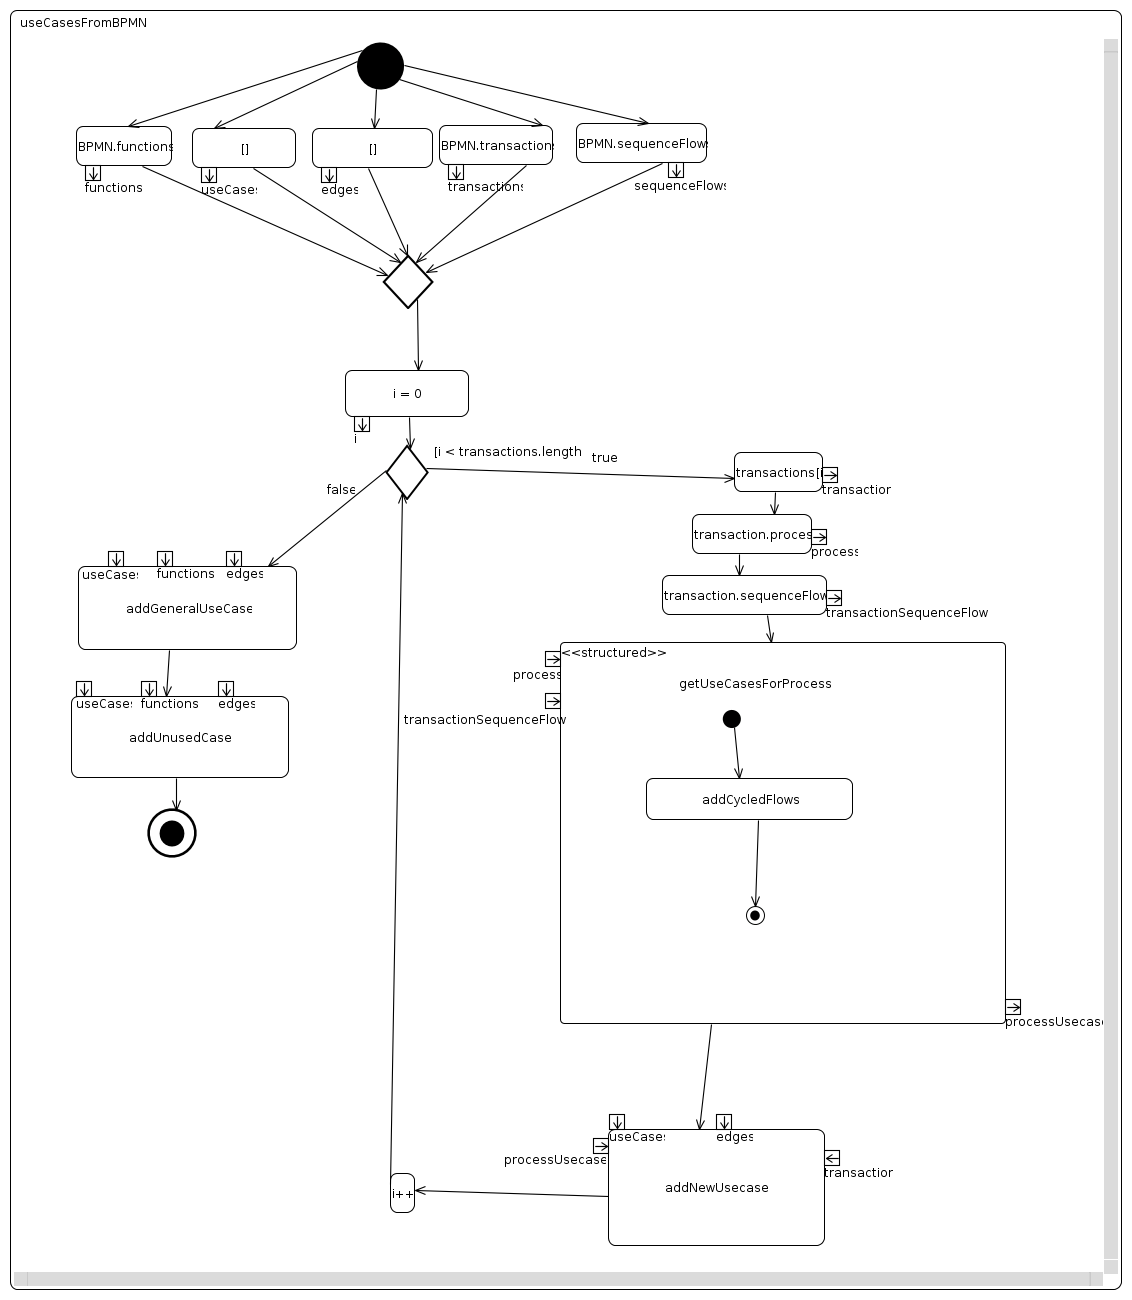
\includegraphics[scale=0.5]{img/algorythm-activity-diagram}
	\label{img:algorythm_activity_diagram}
\end{figure} 

\renewcommand{\lstlistingname}{Pseudokodas}% Listing -> Algorithm
\renewcommand{\lstlistlistingname}{Pseudokodo fragmentai}% List of Listings -> List of Algorithms
\begin{enumerate}
	\item Iškviečiama funkcija useCasesFromBPMN (Pseudokodas \ref{lst:bpmn_to_uc_pseudocode}) paduodant jai \BPMN{} modelį.
	
	\lstinputlisting[style=pseudocode, caption={\UML{} Užduočių diagramos gavimo iš \BPMN{} modelio algoritmo pseudokodas}, label={lst:bpmn_to_uc_pseudocode}]{algorythm-pseudocode/useCasesFromBPMN}
	
	\item Po duomenų inicializavimo pirmiausia imamas transakcijos procesas (eil. \ref{line:bpmn_to_uc_pseudocode_get_process}) ir gaunami sekos srautai jungiantys komponentus transakcijoje (eil. \ref{line:bpmn_to_uc_pseudocode_get_transactionSequenceFlows}). 
	\item Vėliau sukuriami vartojimo atvejai apibrėžiantys proceso valdymą (eil. \ref{line:bpmn_to_uc_pseudocode_get_processUsecases}) funkcija getUseCasesForProcess (Pseudokodas  \ref{lst:bpmn_to_uc_pseudocode_getUseCasesForProcess}).
	
	\lstinputlisting[style=pseudocode, caption={Funkcija getUseCasesForProcess}, label={lst:bpmn_to_uc_pseudocode_getUseCasesForProcess}]{algorythm-pseudocode/getUseCasesForProcess}
	
	\item Joje randami sekos srautai išeinantys iš proceso (eil. \ref{line:bpmn_to_uc_pseudocode_getUseCasesForProcess_get_processFlows}) ir kiekvienam iš jų rekursijos būdu surandami ciklai su procesu funkcija addCycledFlows (Pseudokodas  \ref{lst:bpmn_to_uc_pseudocode_addCycledFlows}). Kiekvienam iš cikle esančių sekos srautų sukuriamas vartojimo atvejis (eil. \ref{line:bpmn_to_uc_pseudocode_getUseCasesForProcess_get_processUsecases_begin} - \ref{line:bpmn_to_uc_pseudocode_getUseCasesForProcess_get_processUsecases_end}). Jų kolekcija ir yra (Pseudokodas  \ref{lst:bpmn_to_uc_pseudocode_getUseCasesForProcess}) grąžinamas rezultatas.
	
	\lstinputlisting[style=pseudocode, caption={Funkcija addCycledFlows}, label={lst:bpmn_to_uc_pseudocode_addCycledFlows}]{algorythm-pseudocode/addCycledFlows}
	
Minėta Funkcija (Pseudokodas  \ref{lst:bpmn_to_uc_pseudocode_addCycledFlows}) pirmiausia patikrina ar jau nėra ciklo su procesu ir jei taip patvirtina, kad parametras currentPath turi savyje kelia į procesą (eil. \ref{line:bpmn_to_uc_pseudocode_addCycledFlows_isTargetProcess_begin} - \ref{line:bpmn_to_uc_pseudocode_addCycledFlows_isTargetProcess_end}). Jei kelias užsiciklino grąžinamas neigiamas atsakymas (eil. \ref{line:bpmn_to_uc_pseudocode_addCycledFlows_isGoingInCircles_begin} - \ref{line:bpmn_to_uc_pseudocode_addCycledFlows_isGoingInCircles_end}), tai reiškia grįžimą atgal. Jei žingsnis veda į jau išsaugotą sėkmingą kelio atkarpą patvirtinamas jo teisingumas (eil. \ref{line:bpmn_to_uc_pseudocode_addCycledFlows_isAlreadyFound_begin} - \ref{line:bpmn_to_uc_pseudocode_addCycledFlows_isAlreadyFound_end}). Jei nei viena iš šių sąlygų nepasitvirtino paimami sekantys žingsniai  (eil. \ref{line:bpmn_to_uc_pseudocode_addCycledFlows_getNextFlows}). Jų neradus pranešama apie aklavietę (eil. \ref{line:bpmn_to_uc_pseudocode_addCycledFlows_isDeadEnd_begin} - \ref{line:bpmn_to_uc_pseudocode_addCycledFlows_isDeadEnd_end}). Kol kas pažymima, kad žingsnis yra sėkmingas (eil. \ref{line:bpmn_to_uc_pseudocode_addCycledFlows_soFarSoGood}) ir žengtas (eil. \ref{line:bpmn_to_uc_pseudocode_addCycledFlows_takeStep}). Toliau ieškoma ciklų su procesu einant sekančiais sekos srautais (eil.  \ref{line:bpmn_to_uc_pseudocode_addCycledFlows_continueRecursion_begin} - \ref{line:bpmn_to_uc_pseudocode_addCycledFlows_continueRecursion_end}). Neradus nei vieno kelio į procesą ištrinamas pažymėjimas apie žingsnio teisingumą (eil.  \ref{line:bpmn_to_uc_pseudocode_addCycledFlows_isPathFound_begin} - \ref{line:bpmn_to_uc_pseudocode_addCycledFlows_isPathFound_end}). Kadangi keliai žengus šį žingsnį ištyrinėti grįžtama atgal (eil. \ref{line:bpmn_to_uc_pseudocode_addCycledFlows_stepBack}).
	\item (Pseudokodas \ref{lst:bpmn_to_uc_pseudocode_getUseCasesForProcess}) sukurti vartojimo atvejai pridedami prie jau gautų vartojimo atvejų kartu su ryšiais tarp jų funkcija addNewUsecases (Pseudokodas  \ref{lst:bpmn_to_uc_pseudocode_addNewUsecases}). 
	
\lstinputlisting[style=pseudocode, caption={Funkcija addNewUsecases}, label={lst:bpmn_to_uc_pseudocode_addNewUsecases}]{algorythm-pseudocode/addNewUsecases}	

Joje sukuriamas vartojimo atvejis visai transakcijai (eil. \ref{line:bpmn_to_uc_pseudocode_addNewUsecases_transactionUseCase}), pažiūrima kiek vartojimo atvejų rasta, jei vienas tai jo informacija išsaugoma į pagrindinį vartojimo atvejį (eil.  \ref{line:bpmn_to_uc_pseudocode_addNewUsecases_onlyMain_begin} - \ref{line:bpmn_to_uc_pseudocode_addNewUsecases_onlyMain_end}). Radus daugiau, jie išsaugomi kaip įeinantys į transakciją (eil.  \ref{line:bpmn_to_uc_pseudocode_addNewUsecases_addIncluded_begin} - \ref{line:bpmn_to_uc_pseudocode_addNewUsecases_addIncluded_end}). 
	\item Galiausiai randamos bendros funkcijos tarp transakcijų ir sukuriami apibendrinantys vartojimo atvejai (Pseudokodas  \ref{lst:bpmn_to_uc_pseudocode_addGeneralUseCases}).
	
	\lstinputlisting[style=pseudocode, caption={Funkcija addGeneralUseCases}, label={lst:bpmn_to_uc_pseudocode_addGeneralUseCases}]{algorythm-pseudocode/addGeneralUseCases}
	
	\item Jeigu liko nepanaudotų funkcijų, iš jų sukuriami vartojimo atvejai su perspėjimais (Pseudokodas \ref{lst:bpmn_to_uc_pseudocode_addUnusedCases}).
	
	\lstinputlisting[style=pseudocode, caption={Funkcija addUnusedCases}, label={lst:bpmn_to_uc_pseudocode_addUnusedCases}]{algorythm-pseudocode/addUnusedCases}
\end{enumerate} 

Sudėtingiausia algoritmo vieta yra transakcijos grafo viršūnių radimas (Pseudokodas  \ref{lst:bpmn_to_uc_pseudocode_addCycledFlows}), kuriam naudojamas paieškos į gylį algoritmas, taigi sudėtingumas yra tiesinis. Atlikusi šio algoritmo veiksmus programa iš \ref{appendix:dvcm_window} priede pavaizduoto vertės grandinės modelio gauna \ref{appendix:use_cases_window} priede pavaizduotą užduočių diagramą.
